\documentclass[t,11pt,british,english, top=1.0in]{beamer}
%\usetheme{amcg}
%\usetheme{iclpt}
\usepackage{url}
\usepackage{hyperref}
\usepackage{graphics}
\usepackage{amsmath}
\usepackage{amssymb}
\usepackage{tikz}
\usetikzlibrary{calc,decorations.pathreplacing}
\usepackage{natbib}
        %You can use the package \textbf{pgfpages} 
        %to arrange your slides for printing. This is also explained
        %in the \textbf{beamer} documentation.

\newcommand{\tensor}[1]{\overline{\overline{#1}}}
\newcommand{\tautens}{\tensor{\tau}}

\setbeamerfont{framesubtitle}{size=\normalsize}
\setbeamerfont{framesubtitle}{size=\normalsize}
%\setbeamertemplate{frametitle}[default][center]
%\setbeamersize{text margin left=6mm}

\usetheme{Madrid}
\usecolortheme{orchid}

%gets rid of bottom navigation bars
\setbeamertemplate{footline}[page number]{}
\setbeamertemplate{headline}{}

%gets rid of navigation symbols
\setbeamertemplate{navigation symbols}{}

\begin{document}
\title{Introduction to programming for Geoscientists\\\vspace*{5mm}Revision Lecture 1}
\author{} 
\date{} 

\frame{\titlepage} 

\frame{
   \frametitle{Variables}
   \framesubtitle{Definition} 
   \begin{itemize}
    \item {\color{red}Variable}: a place in the computer's memory which holds a value.
    \vspace*{2mm}
      \begin{itemize}
        \item Memory {\color{red}address} + symbolic {\color{red}name}\vspace*{1mm}
        \item You define the symbolic name in your Python program.\vspace*{1mm}
        \item e.g. If a variable called \texttt{a} does not already exist, the statement \texttt{a = 5} stores the value 5 in an un-used block of memory.\vspace*{1mm}
        \item The value can then be {\color{red}referenced} (i.e. accessed) using the symbolic name, e.g. \texttt{print a}.
      \end{itemize}
   \end{itemize}
   \vspace*{5mm}
   A simplified view of variable storage:
   \begin{figure}[H]
      \centering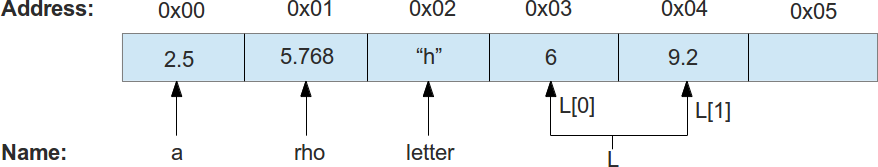
\includegraphics[width=0.9\columnwidth]{images/memory.png}
   \end{figure}
}

\frame{
  \frametitle{Variables}
  \framesubtitle{Key points}
  \begin{itemize}
    \item Always make sure variables are defined \textbf{before trying to use them}! The following block of code will not work:
      \begin{minipage}[t]{.5\textwidth}
        \texttt{b = 5\\ c = a*b\\ a = 10}
      \end{minipage}\vspace*{5mm}
    \item Variable names:\vspace*{1mm}
    \begin{itemize}
      \item are {\color{red}case sensitive}.\vspace*{1mm}
      \item cannot start with a digit.\vspace*{1mm}
      \item cannot be a Python keyword: \texttt{and, as, assert, break, class, continue, def, del, elif, else, except, exec, finally, for, from, global, if, import, in, is, lambda, not, or, pass, print, raise, return, try, with, while, yield}.\vspace*{1mm}
    \end{itemize}
  \end{itemize}
}

\frame{
  \frametitle{Printing}
  \framesubtitle{}
  \begin{itemize}
    \item Data held in variables can be printed to the screen using 
      \begin{minipage}[t]{.5\textwidth}
        \texttt{b = 5.67560\\ print b}
      \end{minipage}\vspace*{2mm}
    \item Or, to present data in a nicer way, use {\color{red}printf style formatting}:
      \begin{minipage}[t]{\textwidth}
        \texttt{print "The data held in variable b is: \%.2f" \% (b)}
      \end{minipage}\vspace*{2mm}
    \item The {\color{red}format specifier} \texttt{\%.2f} acts like a {\color{red}placeholder}. When printing to the screen, Python substitutes this for the data in \texttt{b} and formats it accordingly:
    \begin{itemize}
      \item \texttt{\%.2f} prints out the data in \texttt{b} to 2 decimal places (i.e. \texttt{5.67}).
      \item \texttt{\%d} prints out the data in \texttt{b} as an integer (i.e. \texttt{5}).
      \item \texttt{\%g} prints out the data in \texttt{b} to the minimum number of significant figures (i.e. \texttt{5.6756}).
    \end{itemize}
    \item If you see numbers like \texttt{5e-2}, this is just Python's way of writing $5 \times 10^{-2}$. It has nothing to do with the mathematical constant $e \approx 2.71828$. \vspace*{2mm}
  \end{itemize}
}

\frame{
  \frametitle{Integer division}
  \framesubtitle{}
  \begin{itemize}
    \item In Python, dividing an integer by another integer will result in {\color{red}another integer}.\vspace*{2mm}
    \item Python computes the result, and {\color{red}drops the decimal point and everything after it}. e.g. 9/5 = 1.8 will evaluate to 1\vspace*{2mm}
    \item This is a common error made in Python programs, so watch out for it.\vspace*{2mm}
    \item If in doubt, just make the numerator or denominator (or both) floating-point numbers. e.g. 3 $\rightarrow$ 3.0\vspace*{2mm}
  \end{itemize}
}

\frame{
  \frametitle{Variable type conversion}
  \framesubtitle{}
  \begin{itemize}
    \item Converting a variable's data from one type to another.\vspace*{2mm}
    \begin{itemize}
      \item \texttt{int(5.0)} $\rightarrow$ \texttt{5}
      \item \texttt{float(7)} $\rightarrow$ \texttt{7.0}
      \item \texttt{str(8.15)} $\rightarrow$ ``\texttt{8.15}''
      \item \texttt{int("5")} $\rightarrow$ \texttt{5}
    \end{itemize}
    \item Also known as {\color{red}type casting}.\vspace*{2mm}
    
    \item You will most likely use casting:
    \begin{itemize}
      \item to avoid integer division problems, e.g. \texttt{float(3)/5}
      \item when you want to use numerical data read in from the keyboard using \texttt{raw\_input}, e.g. 
      \begin{minipage}[t]{\textwidth}
        \texttt{a = 5\\ b = raw\_input("Please enter a number.")\\ c = a*float(b)}
      \end{minipage}\vspace*{2mm}
    \end{itemize}
    
  \end{itemize}
}

\frame{
  \frametitle{Operator precedence}
  \framesubtitle{}
  \begin{itemize}
    \item Expressions like \texttt{2.0 + 3.0/5.0} are evaluated in a particular order, determined by {\color{red}operator precedence}.\vspace*{2mm}
    \item Division has a {\color{red}higher precedence} than addition, so \texttt{3.0/5.0} is evaluated {\color{red}first}, and \texttt{2.0} is then added on afterwards.\vspace*{2mm}
    \item If we wanted \texttt{2.0 + 3.0} to be evaluated first, then we need to use {\color{red}parentheses}: \texttt{(2.0 + 3.0)/5.0}.\vspace*{2mm}
    \item {\color{red}BODMAS}: {\color{red}B}rackets, {\color{red}O}rder, {\color{red}D}ivision, {\color{red}M}ultiplication, {\color{red}A}ddition, {\color{red}S}ubtraction.
    \newline
    \item Note: Python groups certain operators together such that they have the same precedence, and then evaluates expressions from left to right. See \texttt{http://docs.python.org/2/reference/expressions.html}.
  \end{itemize}
}

\frame{
  \frametitle{Importing modules}
  \framesubtitle{}
  \begin{itemize}
    \item Python {\color{red}modules} are useful when you want to split your code up to make it more manageable, or to make a piece of code available for use in other programs.\vspace*{2mm}
    \item Mathematical functions like $\sin(x)$, $\cos(x)$, $\log(x)$ are available in the \texttt{math} module.\vspace*{2mm}
    \item There are two ways of importing functions from modules:\vspace*{2mm}
    \begin{itemize}
      \item \texttt{import math}: Python will import all the functions in the math module, but will keep the functions in their own separate {\color{red}namespace}. That is, you must use {\color{red}prepend \texttt{math.} to the function's name} to use it, e.g. \texttt{x = 0.5; y = math.sin(x)}\vspace*{2mm}
      \item \texttt{from math import *}: Python will import all the functions in the math module into the current namespace. That is, you can simply do \texttt{x = 0.5; y = sin(x)}. But: be careful that you do not have another function named \texttt{sin} in your program!
    \end{itemize}
  \end{itemize}
}

\frame{
  \frametitle{If statement}
  \framesubtitle{Definition}
  \begin{itemize}
    \item The {\color{red}if statement} is a programming construct that executes different blocks of code depending on whether a boolean {\color{red}condition} evaluates to {\color{red}\texttt{True}} or {\color{red}\texttt{False}}.\vspace*{2mm}
    
    \begin{minipage}[t]{\textwidth}
       \texttt{if(boolean condition):}
    
       \ \ \ \ \ \indent\texttt{print "The condition is True"}
       
       \texttt{else:}
           
       \ \ \ \ \ \indent\texttt{print "The condition is False"}
    \end{minipage}\vspace*{2mm}
    \vspace*{2mm}
    \item Condition: it is raining (True or False)
    \item Possible actions: take an umbrella, don't take an umbrella.
    \begin{minipage}[t]{\textwidth}
       \texttt{if(it is raining):}
    
       \ \ \ \ \ \indent\texttt{Take an umbrella.}
       
       \texttt{else:}
           
       \ \ \ \ \ \indent\texttt{Don't take an umbrella.}
    \end{minipage}\vspace*{2mm}
  \end{itemize}

}

\frame{
  \frametitle{If statements}
  \framesubtitle{Examples of conditions}
  \begin{itemize}
  \item \texttt{b = 40}\vspace*{2mm}
  \item {\color{red}Equality} condition: \texttt{b == 40} $\rightarrow$ \texttt{True}\vspace*{2mm}
  \item {\color{red}Negation} (also known as the logical complement):\\\texttt{b != 40} $\rightarrow$ \texttt{False}\\
        \texttt{not(b == 40)} $\rightarrow$ \texttt{False}\vspace*{2mm}\\
  \item {\color{red}Or} condition: \texttt{b >= 40} $\rightarrow$ \texttt{True}\\
        \texttt{b == 40 or b > 40} $\rightarrow$ \texttt{True}\vspace*{2mm}\\
  \item {\color{red}And} condition: \texttt{b > 30 and b < 70} $\rightarrow$ \texttt{True}\\
                      \texttt{b > 30 and b < 35} $\rightarrow$ \texttt{False}
  \end{itemize}
}

\frame{
  \frametitle{Logicals}
  \framesubtitle{And}
   \begin{figure}[H]
      \centering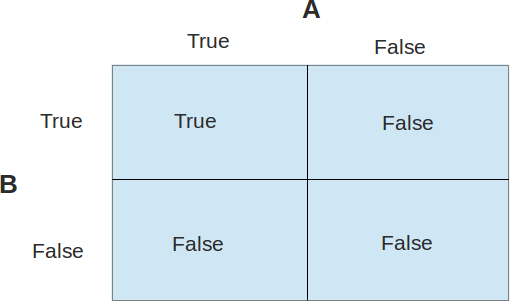
\includegraphics[width=0.9\columnwidth]{images/logical_and.png}
   \end{figure}
}

\frame{
  \frametitle{Logicals}
  \framesubtitle{Or}
   \begin{figure}[H]
      \centering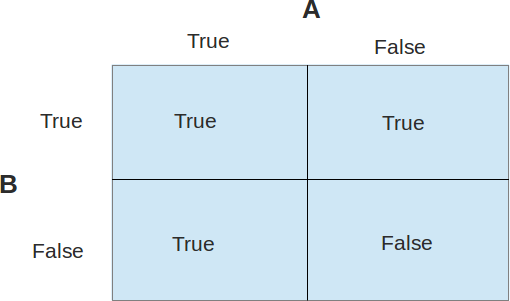
\includegraphics[width=0.9\columnwidth]{images/logical_or.png}
   \end{figure}
}

\frame{
  \frametitle{Lists}
  \framesubtitle{Definition}
  \begin{itemize}
    \item {\color{red}List}: a Python data structure that can hold a {\color{red}sequence} of {\color{red}elements}/items/values. Elements can be added to, or removed from, a list.\vspace*{2mm}
    \item A list can be defined by enclosing the elements (separated by {\color{red}commas}) in {\color{red}square brackets}, e.g. \texttt{L = [4, 6, 2, -1]}\vspace*{2mm}
    \item {\color{red}Append} an element to the end of a list by using the general form: \texttt{list\_name.append(value)}\vspace*{2mm}
    \item Get the length of a list using the {\color{red}\texttt{len} function}: \texttt{len(L)} returns a value of 4.
  \end{itemize}
}

\frame{
  \frametitle{Lists}
  \framesubtitle{Referencing elements}
  \begin{itemize}
    \item Each element of the list is assigned an {\color{red}index}, with the first element's index being zero.\vspace*{2mm}
    \item To reference/access an element of the list, follow the general form: {\color{red}\texttt{list\_name[element\_index]}}
    \begin{itemize}
      \item \texttt{L[0]} $\rightarrow$ \texttt{4}
      \item \texttt{L[-1]} $\rightarrow$ \texttt{-1}
      \item \texttt{L[len(L)-1]} $\rightarrow$ \texttt{-1}
    \end{itemize}
  \end{itemize}
  \begin{figure}[H]
      \centering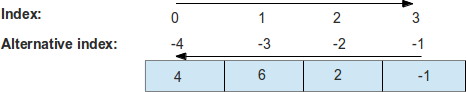
\includegraphics[width=0.9\columnwidth]{images/list.png}
  \end{figure}
}


\frame{
  \frametitle{Lists}
  \framesubtitle{Slicing}
  \begin{itemize}
    \item Sub-lists can also be extracted from a list. This is known as {\color{red}slicing}.\vspace*{2mm}
    \item General usage: \texttt{list\_name[start\_index:end\_index]}. By default, \texttt{start\_index} is implicitly set to 0 if not provided by the user. Similarly, \texttt{end\_index} is implicitly set to \texttt{len(list\_name)} if not provided.\vspace*{2mm}
    \item \texttt{L[0:len(L)]} $\equiv$ \texttt{L[:]} $\equiv$ \texttt{L}\vspace*{2mm}
    \item Example: \texttt{L = [2, 5, 8, 0, 5, 1]}.\\ \texttt{A = L[:4]} $\rightarrow$ \texttt{A = [2, 5, 8, 0]}.
  \end{itemize}
}

\frame{
  \frametitle{Lists}
  \framesubtitle{Zip two lists}
  \begin{itemize}
    \item Elements from two lists can be combined using the {\color{red}zip} function to form a new list: a {\color{red}list of tuples}.
  \end{itemize}
  \begin{figure}[H]
      \centering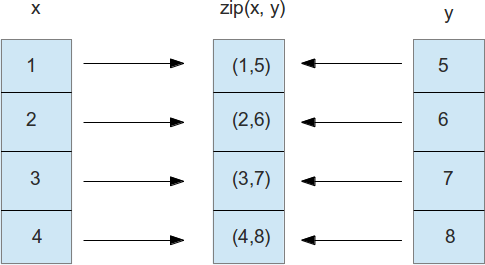
\includegraphics[width=0.9\columnwidth]{images/zip.png}
  \end{figure}
}

\frame{
  \frametitle{Loops}
  \framesubtitle{Definition}
  \begin{itemize}
    \item {\color{red}Loop}: a programming construct that allows a block of code to be executed multiple times.\vspace*{2mm}
    \item Two types of loop: {\color{red}\texttt{while}} and {\color{red}\texttt{for}}.
  \end{itemize}
}

\frame{
  \frametitle{Loops}
  \framesubtitle{While loop}
  \begin{itemize}
    \item Iterate indefinitely while some boolean condition is \texttt{True}. This condition is called the {\color{red}loop invariant}.\vspace*{2mm}
    \item The invariant is evaluated before the start of each iteration. If it evaluates to True, Python executes all the statements in the indented code block.\vspace*{2mm}
    \item General form:
    \begin{minipage}[t]{\textwidth}
       \texttt{while(boolean condition is True):}
    
       \ \ \ \ \ \indent\texttt{Statements to be executed}
       
       \ \ \ \ \ \indent\texttt{within a single loop iteration}.
    \end{minipage}\vspace*{2mm}
    \item Remember to update any variables that the boolean condition depends on within the loop, e.g. if the condition is \texttt{i < 100}, you might do \texttt{i = i + 1}. Otherwise, \texttt{i} will never increase, the boolean condition will always be True, and the loop will never end.
  \end{itemize}
}

\frame{
  \frametitle{Loops}
  \framesubtitle{For loop}
  \begin{itemize}
    \item For loops must have {\color{red}something to iterate over}. This is usually a list or an array.
    \item General form of a \texttt{for} loop:
    \begin{minipage}[t]{\textwidth}
       \texttt{for {\color{red}iterator} in {\color{red}iterable\_object}:}
       
       \ \ \ \ \ \indent\texttt{Do some cool stuff, possibly involving the iterator.}
    \end{minipage}\vspace*{2mm}
    \item Example:
      \begin{itemize}
        \item Iterator: \texttt{i}
        \item Iterable object: \texttt{range(0, 3)} $\rightarrow$ \texttt{[0, 1, 2]}
        \begin{minipage}[t]{\textwidth}
        \texttt{for i in range(0, 3):}
       
        \ \ \ \ \ \indent\texttt{print i*2}
        
        \texttt{print "Out of the loop!"}
        \end{minipage}\vspace*{2mm}
        \item Iteration 1: \texttt{i} = 0, Python prints out 0 to the screen.$\curvearrowright$
        \item Iteration 2: \texttt{i} = 1, Python prints out 2 to the screen.$\curvearrowright$
        \item Iteration 3: \texttt{i} = 2, Python prints out 4 to the screen.$\curvearrowright$
        \item No more elements to iterate over, so the loop ends.
        \item Python prints \texttt{"Out of the loop!"}
      \end{itemize}
  \end{itemize}
}

\frame{
  \frametitle{Functions}
  \framesubtitle{Definition}
  \begin{itemize}
    \item {\color{red}Function}: a programming construct that expects zero or more {\color{red}inputs}, and returns zero or more {\color{red}outputs}.\vspace*{2mm}
    \item General form:\vspace*{2mm}
        \begin{minipage}[t]{\textwidth}
        \texttt{def function\_name(input1, input2):}
       
        \ \ \ \ \ \indent\texttt{The function's {\color{red}body}. Compute any output values here.}
        
        \ \ \ \ \ \indent\texttt{return output1, output2, output3}
        \end{minipage}\vspace*{2mm}
    \item The inputs are known as {\color{red}arguments}.\vspace*{2mm}
    \item Example: the function \texttt{len} takes in 1 argument (a list/tuple/string/...) and returns 1 value (the length of that list/tuple/string).
  \end{itemize}
}

\frame{
  \frametitle{User input}
  \framesubtitle{}
  \begin{itemize}
    \item User input can be read from the keyboard using the {\color{red}\texttt{raw\_input}} function. This takes 1 argument (a message that you want to show to the user, e.g. ``Enter a number between 1 and 10''), and gives 1 output (the user's input).\vspace*{2mm}
    \item This return/output value of the \texttt{raw\_input} function is always a {\color{red}string}. \vspace*{2mm}
    \item Remember: numerical data in string form needs to be {\color{red}converted}, or {\color{red}casted}, to a float or integer.\vspace*{2mm}
  \end{itemize}
}


\frame{
  \frametitle{Exception handling}
  \framesubtitle{Definition}
  \begin{itemize}
    \item {\color{red}Exceptions}: errors that occur when Python cannot properly execute a line of code at run-time.\vspace*{2mm}
    \item Common examples include:
    \begin{itemize}
      \item Trying to reference an element in a list that doesn't exist. e.g. \texttt{L = [1, 2]; print L[2]}
      \item Trying to divide by zero.
    \end{itemize}\vspace*{2mm}
    \item It is important that we handle these errors {\color{red}gracefully}, because:
    \begin{itemize}
       \item The standard exception error message will probably confuse an average user.
       \item The program might not be able to continue executing properly.
    \end{itemize}\vspace*{2mm}
  \end{itemize}
}

\frame{
  \frametitle{Exception handling}
  \framesubtitle{try-except blocks}
  \begin{itemize}
    \item {\color{red}try-except blocks} are used to handle exceptions.\vspace*{2mm}
    \item Identify lines of your code where an exception may occur, and wrap them in a \texttt{try} block.\vspace*{2mm}
    \item In the \texttt{except} block, we decide how to handle the error. e.g.
    \begin{minipage}[t]{\textwidth}
        \texttt{try:}
        
        \ \ \ \ \ \indent\texttt{number = float(raw\_input("Enter a number:")}
        
        \texttt{except ValueError:}
        
        \ \ \ \ \ \indent\texttt{print "Error: you didn't enter a number."}
    \end{minipage}\vspace*{2mm}
  \end{itemize}
}

\end{document}
